%%%%%%%%%%%%%%%%%%%%%%%%%%%%%%%%%%%%%%%%%%%%%%%%%%%%%%%%%%%%%%%%%%%%%%%%%%%%%%%
%%  ClaudeNet v3 -- image atlas of the Table 11 grade-A survivors.
%%  These are NEW to the Huang/Storfer/Inchausti lineage but, on a literature
%%  (NED/SIMBAD) crossmatch, are rediscoveries of known lenses (CASSOWARY/DES/AGEL).
%%  Standalone report (sibling of main.tex). Figures from ../93_make_gallery.py;
%%  the literature crossmatch from ../94_external_xmatch.py.
%%%%%%%%%%%%%%%%%%%%%%%%%%%%%%%%%%%%%%%%%%%%%%%%%%%%%%%%%%%%%%%%%%%%%%%%%%%%%%%
\documentclass[11pt,letterpaper]{article}
\usepackage{../../tech-report}
\usepackage{graphicx}

\newcommand{\cnet}{\textsc{ClaudeNet}}
\newcommand{\plens}{\ensuremath{p_{\rm lens}}}

\title{\cnet{} v3: Three DR10 Grade-A Lenses New to the Huang/Storfer/Inchausti\\
       Lineage --- Rediscoveries of Known Strong Lenses}
\author{Greg Benson\thanks{\texttt{benson@cs.usfca.edu}; Department of Computer
        Science, University of San Francisco, CA 94117, USA} \and
        Xiaosheng Huang\thanks{Department of Physics \& Astronomy, University of
        San Francisco; and Physics Division, Lawrence Berkeley National Laboratory}}
\date{June 2026}

\begin{document}
\maketitle
\subtitle{Each is a previously-published lens (CASSOWARY, DES, AGEL) recovered independently by v3 at DESI resolution --- external validation, not net-new discovery}

\section{Three grade-A lenses, new to the lineage --- all rediscoveries}
\cnet{}~v3's DR10 contaminant-aware vetting (C-vet) surfaced three grade-A
candidates that the \emph{lineage} crossmatch --- Storfer 2024, Inchausti 2025,
and Huang 2020/2021 --- reported as absent from the catalogued sample, i.e.\
``new'' (Table~11 of \texttt{papers/main.pdf}). A literature-wide NED/SIMBAD
crossmatch (\texttt{94\_external\_xmatch.py}), however, shows that each coincides
to within $\le0.5\arcsec$ with a previously-published strong lens found by
\emph{another} survey. They are therefore independent \textbf{rediscoveries}, not
net-new discoveries --- a genuine external validation that v3 recovers real lenses
at DESI resolution, but not new objects. (A fourth C-vet survivor,
\texttt{s\_310364\_6649}, is the Huang+2020 grade-A lens
\texttt{DESI-038.2078-03.3906}; it is handled in the main report.)

The cutouts below are the DECaLS grz imaging at the finder's native geometry
($101$\,px, $0.262\arcsec$/px), fetched and rendered with the group's
inspection-viewer renderer (Lupton $Q{=}8$, $400$\,px upsample) by
\texttt{93\_make\_gallery.py} --- the exact pixels the v3 model and the panel saw.
For each object we show the \emph{full} cutout, a $2.5\times$ center \emph{zoom},
and a lens-light-subtracted \emph{residual} that exposes the arc/ring.

\paragraph{Honest framing.} The net-new count from this set is \textbf{zero}: all
three (and the Huang+2020 object) are known lenses. The value is external
validation, not discovery. These positions have \emph{no} Euclid coverage, and
net-new discovery at DESI's $\sim$$1.3\arcsec$ seeing remains resolution-bounded.

\begin{table}[h]\centering
\caption{The three v3 grade-A C-vet survivors that are new to the
Huang/Storfer/Inchausti lineage, with the previously-published lens each
rediscovers (literature NED/SIMBAD crossmatch, \texttt{94\_external\_xmatch.py}).}
\label{tab:newcand}\small
\begin{tabular}{lccclc}
\toprule
DESI id & RA (deg) & Dec (deg) & C-vet \plens{} & rediscovered lens (survey) & sep\\
\midrule
s\_441355\_1111  & $177.1381$ & $+19.5009$ & 0.74 & CSWA 1 (CASSOWARY)             & $0.5\arcsec$\\
s\_124958\_10481 & $58.1768$  & $-38.4292$ & 0.82 & DES J0352$-$3825 (DES)         & $0.2\arcsec$\\
s\_102952\_9916  & $334.8017$ & $-43.8098$ & 0.76 & AGEL J221912$-$434835 (AGEL/DES) & $0.2\arcsec$\\
\bottomrule
\end{tabular}
\end{table}

\section{Cutout panels}

\begin{figure}[!ht]\centering
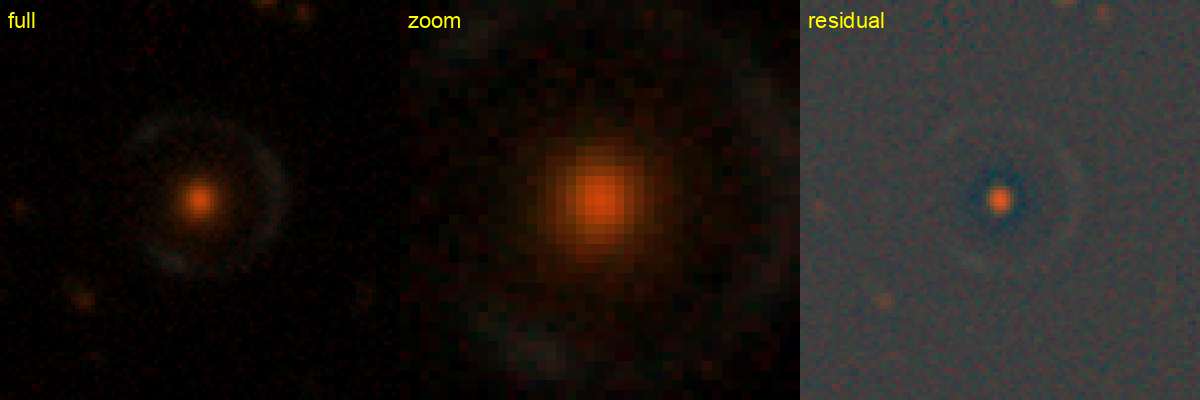
\includegraphics[width=0.95\linewidth]{figures/newcand_s_441355_1111.png}
\caption{\textbf{s\_441355\_1111} --- RA $177.1381\degr$, Dec $+19.5009\degr$;
C-vet \plens{}$=0.74$. \textbf{Rediscovery of CSWA~1 --- the Cosmic Horseshoe}
(CASSOWARY survey; Belokurov et al.\ 2007), a near-complete Einstein ring around a
massive LRG. Literature match $0.1$--$0.5\arcsec$ (SIMBAD CSWA~1 and its lensed
images). Panels: full / zoom ($2.5\times$) / lens-light residual.}
\label{fig:c1}
\end{figure}

\begin{figure}[!ht]\centering
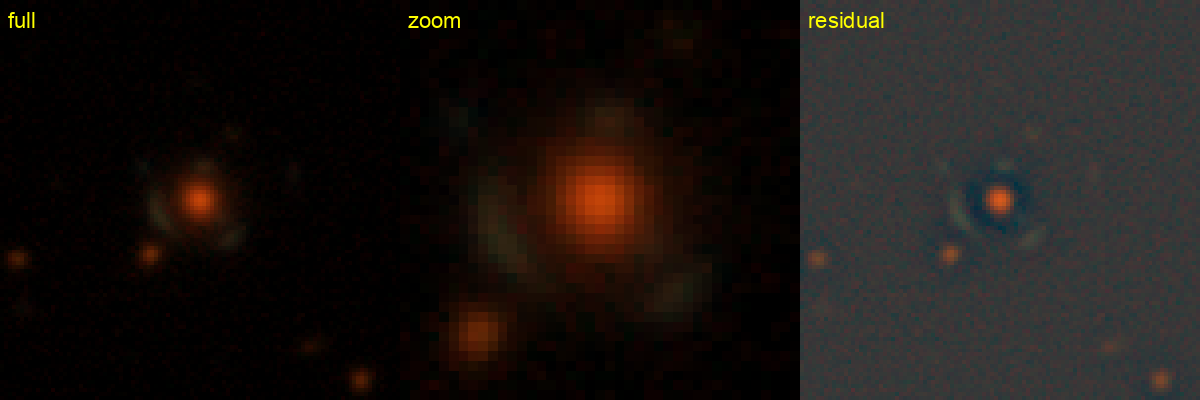
\includegraphics[width=0.95\linewidth]{figures/newcand_s_124958_10481.png}
\caption{\textbf{s\_124958\_10481} --- RA $58.1768\degr$, Dec $-38.4292\degr$;
C-vet \plens{}$=0.82$. \textbf{Rediscovery of DES~J0352$-$3825} (Dark Energy
Survey; O'Donnell et al.\ 2022). Literature match $0.2\arcsec$ to the lens galaxy;
NED lists three lensed images at $2.6$--$3.7\arcsec$. Panels: full / zoom
($2.5\times$) / lens-light residual.}
\label{fig:c2}
\end{figure}

\begin{figure}[!ht]\centering
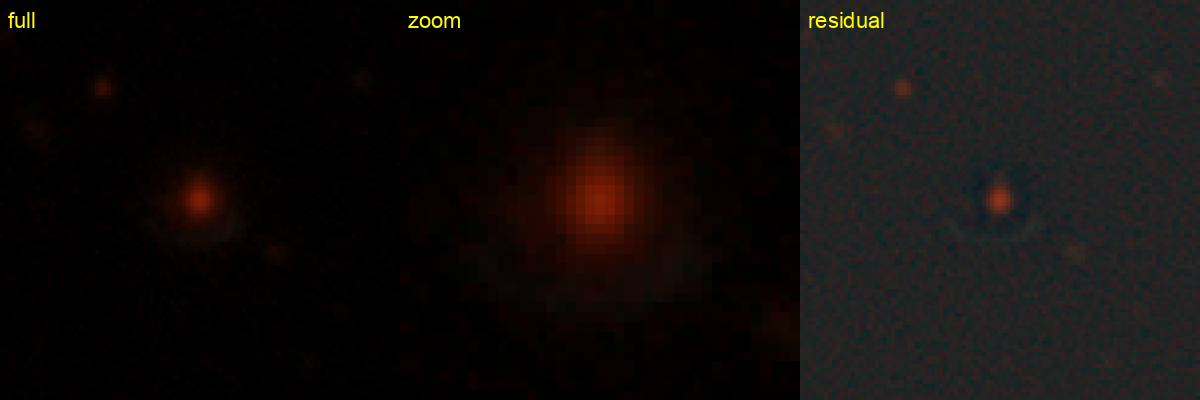
\includegraphics[width=0.95\linewidth]{figures/newcand_s_102952_9916.png}
\caption{\textbf{s\_102952\_9916} --- RA $334.8017\degr$, Dec $-43.8098\degr$;
C-vet \plens{}$=0.76$. \textbf{Rediscovery of AGEL~J221912$-$434835} (AGEL survey,
Keck-confirmed; Tran et al.\ 2022; also DES~J221912.39$-$434835.1). Literature
match $0.2\arcsec$. The residual panel surfaces a near-complete blue ring around
the red elliptical core. Panels: full / zoom ($2.5\times$) / lens-light residual.}
\label{fig:c3}
\end{figure}

\end{document}
